\chapter{Introduction :Pourquoi vous devez utiliser GPG ?}

Quand j'écris des courriels ou que je montre ma carte de visite, il y a
des gens qui me demandent : c'est quoi GPG ? C'est quoi ce fichier en
pièce joint de votre courriel ?

\begin{figure}[h]
\centering
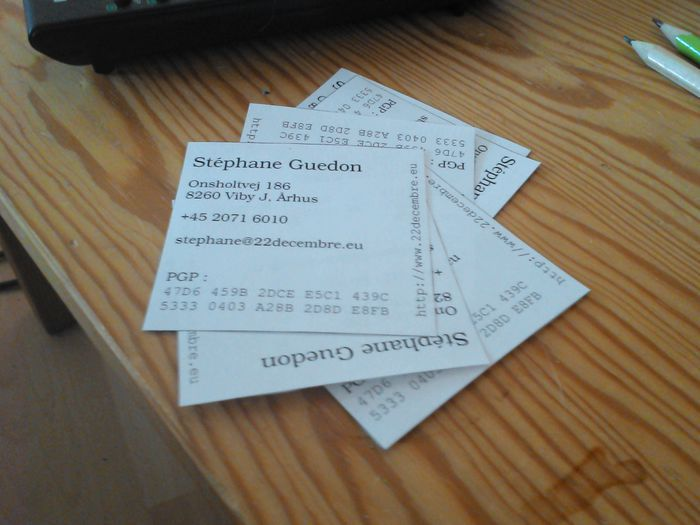
\includegraphics[width=0.7\linewidth]{images/visiting.jpeg}
\caption{Des cartes de visites comportant une empreinte de clé GPG}
\end{figure}

Je suis toujours aussi surpris qu'après les révélations d'Edward 
Snowden\footnote{\url{https://fr.wikipedia.org/wiki/Révélations_d'Edward_Snowden}} sur la surveillance de masse des services secrets américains (NSA, CIA\ldots{}), et les découvertes, chaque jour de l'étendue et des pouvoirs des services secrets occidentaux\footnote{\url{http://www.lemonde.fr/pixels/article/2015/02/17/un-nouveau-logiciel-espion-de-la-nsa-mis-au-jour_4577707_4408996.html}} - y compris français -, il y ait des gens (la \emph{majorité} des gens en fait, aussi triste que ça puisse
paraître !) qui ne connaissent pas GPG !

Je me suis donc décidé à publier ce puis un tutoriel au long court qui j'espère, vous permettront d'apprendre à l'utiliser correctement.

\section{La démarche}\label{la-duxe9marche}

À l'opposé de la plupart des tutoriels que vous trouverez sur le net à
propos de GPG, je vais m'efforcer de vous donner les points importants
progressivement, de sorte que vous preniez le temps d'assimiler tout
cela.

En effet, il est inutile, si ce n'est dangereux de vous montrer comment
créer des clés de chiffrement, de vous mener par la main sur tout le
chemin et de vous lâcher dans la nature au bout, à peine deux jours
après vous avoir mis dans le bain.

Il vaut mieux être bien plus progressif. Vous faire réflechir et vous
donner les liens pour comprendre et vous permettre d'approfondir votre
apprentissage et votre compréhension.

\section{C'est quoi GPG ?}\label{cest-quoi-gpg}

\subsection{Tout d'abord il y eu PGP}\label{tout-dabord-il-y-eu-pgp}

PGP est un sigle pour \emph{Pretty Good Privacy}, \emph{Plutôt Bonne Vie Privée} en français.

PGP est le logiciel originel, conçu par Philip Zimmermann\footnote{\url{http://philzimmermann.com/FR/background/index.html}}, dans le
but explicite de défendre la vie privée, les libertés individuelles et plus largement la démocratie\footnote{\url{http://openpgp.vie-privee.org/pourquoi.htm}}. C'est à la base un outil permettant de signer et chiffrer sa correspondance électronique. En français, son mail ou son courriel.

Ce mot, \emph{chiffrement}, il est très important : il indique que l'on
fait appel ici à des mathématiques de très haut niveau, avec des
concepts et des algorithmes complexes.\\Pas d'inquiétude toutefois !
C'est le logiciel lui-même qui fait ces opérations mathématiques.

\subsection{Puis OpenPGP}\label{puis-openpgp}

Puis l'IETF, a normalisé PGP et ça a donné le format de chiffrement OpenPGP\footnote{\url{https://fr.wikipedia.org/wiki/OpenPGP}}, qui garantit que
les différents utilisateurs du format peuvent échanger grâce à ce même format d'échanges.

\subsection{Finalement est venu GPG}\label{finalement-est-venu-gpg}

Ceci a permis à des développeurs libristes de concevoir un logiciel, GnuPG
\footnote{\url{https://www.gnupg.org/}}, abrégé en GPG, implémentant le format OpenPGP. Autrement dit : grâce à OpenPGP, les utilisateurs de
GnuPG et PGP peuvent correspondre ensemble sans problème.

\section{Pourquoi l'utiliser ?}\label{pourquoi-lutiliser}

Vous êtes en couple ? Votre femme (ou votre homme \ldots{}) vous envoie
des photos osées pour vous exciter, ou plus simplement vous échangez des
propos classés X, que vous ne souhaiteriez surtout pas laisser à
disposition du premier venu !

Vous avez une compétition de cuisine et voulez partager votre recette de la tarte au citron avec Bree Hodges, mais pas avec Katherine Mayfair ?

Vous voulez monter une entreprise, ou vous travaillez déjà, et souhaiter donc communiquer en toute sécurité avec vos associés ?

Vous êtes journaliste et voulez communiquer de manière sécurisée avec vos sources ? Ce cas est
particulier, puisqu'idéalement, vos sources doivent pouvoir, dès le départ, sans même vous connaître, communiquer avec vous de manière
confidentielle ! Il est à noter que ce fut le cas d'Edward Snowden : il a utilisé PGP et demandé à ses contacts de faire de même pour assurer
des échanges sûrs.

Certaines de ces raisons semblent futiles. Mais ce que \emph{Desperate Housewives}, et les gens autour de nous, nous ont bel et bien montré,
c'est que, aussi futile que ce soit, quelqu'un peut néanmoins être assez motivé pour vouloir ouvrir votre courrier et dans ce cas, cette personne
mettra aussi en œuvre les moyens les plus importants, et parfois de manière totalement disproportionnée.\\

Mais passons à autre chose\ldots{}
Ouuuuiiii\ldots{}\\

Google\footnote{\url{http://www.linformaticien.com/actualites/id/32860/google-lit-vos-mails-et-assume.aspx}},
Yahoo\footnote{\url{http://www.zdnet.fr/actualites/yahoo-lit-les-emails-de-ses-utilisateurs-quoi-de-neuf-doc-39791003.htm}}
et Microsoft\footnote{\url{http://www.numerama.com/magazine/33357-windows-10-microsoft-et-vos-donnees-privees-ce-que-vous-devez-savoir.html}} lisent vos courriels pour faire du profilage ! Vous rappelez-vous de ce scandale, avec des photos de stars de cinéma volées\footnote{\url{http://www.huffingtonpost.fr/2014/09/02/jennifer-lawrence-nue-piratage-internet-kate-upton-photos-celebgate_n_5745970.html}} ?\\Si vous estimez que la reaction de ces stars (indignation devant les violations de leur vie privée) est
normale, saine, pourquoi n'accordez-vous pas la même valeur à votre vie privée aussi ?\\
\\
Bonne nouvelle toutefois, GPG est toujours sûr apparament
\footnote{\url{http://www.ginjfo.com/actualites/politique-et-economie/espionnage-nsa-depose-les-armes-devant-certaines-solutions-cryptage-20141230}} !\\
\\
D'ailleurs, pour vous donner une autre raison d'utiliser GPG : le mail, à la base, c'est du texte. Rien de plus simple à intercepter, lire,
détourner. En fait, envoyer un mail, c'est envoyer une carte postale ! Ça va bien pour parler des photos du chat, mais très rapidement, ça
devient critique\ldots{} Non ?

\section{C'est douloureux ?}\label{cest-douloureux}

Disons que l'utilisation du chiffrement n'est pas forcement hyper-simple. Toutefois, je ne vois aucun moyen, ni
aucune raison sérieuse de s'en passer.

En mettant à disposition de tous un tutoriel perenne, en vous
permettant, progressivement, de découvrir le fonctionnement d'OpenPGP,
j'espère vous permettre et vous encourager à proteger votre vie privée
et vos libertés individuelles, et celles des personnes qui vous sont
chères. Vous verrez qu'après un peu d'entrainement, l'utilisation de cet outil
devient très vite naturel.